\documentclass[a4paper,10pt]{article} % Uses article class in A4 format

\setlength{\parskip}{0pt}
\setlength{\parindent}{0pt}
\setlength{\voffset}{-15pt}

\usepackage[a4paper, margin=2.5cm]{geometry} % Sets margin to 2.5cm for A4 Paper
\usepackage[onehalfspacing]{setspace} % Sets Spacing to 1.5

\usepackage[T1]{fontenc} % Use European encoding
\usepackage[utf8]{inputenc} % Use UTF-8 encoding
\usepackage{charter} % Use the Charter font
\usepackage{microtype} % Slightly tweak font spacing for aesthetics

\usepackage[english, ngerman]{babel} % Language hyphenation and typographical rules

\usepackage{amsthm, amsmath, amssymb} % Mathematical typesetting
\usepackage{marvosym, wasysym} % More symbols
\usepackage{float} % Improved interface for floating objects
\usepackage[final, colorlinks = true, 
            linkcolor = black, 
            citecolor = black,
            urlcolor = black]{hyperref} % For hyperlinks in the PDF
\usepackage{graphicx, multicol} % Enhanced support for graphics
\usepackage{xcolor} % Driver-independent color extensions
\usepackage{rotating} % Rotation tools
\usepackage{listings, style/lstlisting} % Environment for non-formatted code, !uses style file!
\usepackage{pseudocode} % Environment for specifying algorithms in a natural way
\usepackage{style/avm} % Environment for f-structures, !uses style file!
\usepackage{booktabs} % Enhances quality of tables

\usepackage{tikz-qtree} % Easy tree drawing tool
\tikzset{every tree node/.style={align=center,anchor=north},
         level distance=2cm} % Configuration for q-trees
\usepackage{style/btree} % Configuration for b-trees and b+-trees, !uses style file!

\usepackage{titlesec} % Allows customization of titles
\renewcommand\thesection{\arabic{section}.} % Arabic numerals for the sections
\titleformat{\section}{\large}{\thesection}{1em}{}
\renewcommand\thesubsection{\alph{subsection})} % Alphabetic numerals for subsections
\titleformat{\subsection}{\large}{\thesubsection}{1em}{}
\renewcommand\thesubsubsection{\roman{subsubsection}.} % Roman numbering for subsubsections
\titleformat{\subsubsection}{\large}{\thesubsubsection}{1em}{}

\usepackage[all]{nowidow} % Removes widows

\usepackage[backend=biber,style=numeric,
            sorting=nyt, natbib=true]{biblatex} % Complete reimplementation of bibliographic facilities
\addbibresource{main.bib}
\usepackage{csquotes} % Context sensitive quotation facilities

\usepackage[yyyymmdd]{datetime} % Uses YEAR-MONTH-DAY format for dates
\renewcommand{\dateseparator}{-} % Sets dateseparator to '-'

\usepackage{fancyhdr} % Headers and footers
\pagestyle{fancy} % All pages have headers and footers
\fancyhead{}\renewcommand{\headrulewidth}{0pt} % Blank out the default header
\fancyfoot[L]{\textsc{ModuleShorthand00}} % Custom footer text
\fancyfoot[C]{} % Custom footer text
\fancyfoot[R]{\thepage} % Custom footer text

\newcommand{\note}[1]{\marginpar{\scriptsize \textcolor{red}{#1}}} % Enables comments in red on margin

%----------------------------------------------------------------------------------------

\begin{document}

%----------------------------------------------------------------------------------------
%	TITLE SECTION
%----------------------------------------------------------------------------------------

\title{template_assignment} % Article title
\fancyhead[C]{}
\begin{minipage}{0.295\textwidth} % Left side of title section
\raggedright
\hfill\\ % Uncomment if right minipage has more lines
\medskip\hrule
\end{minipage}
\begin{minipage}{0.4\textwidth} % Center of title section
\centering 
\large % Title text size
Lab 1\\ % Assignment subtitle
\normalsize % Subtitle text size
Introduction to Python, Git, and GitHub\\
\end{minipage}
\begin{minipage}{0.295\textwidth} % Right side of title section
\raggedleft
\hfill\\ % Uncomment if left minipage has more lines
\medskip\hrule
\end{minipage}

\bigskip

\printbibliography

\section{Setting Up Python}

The labs in this course will take place on Anchor days and offer you a chance
to exercise the material in a more traditional setting. Early on in the
semester we will cover the basics of the Git version control system as well as
how to run Python scripts locally.\\

For the labs please download one of the following editors, or any other editor
of your choice, to your machine:

\begin{itemize}
  \item VScode
  \item Atom
  \item vim
  \item sublime 3
  \item GNU Emacs
\end{itemize}

Additionally, please ensure the latest version of Python is installed to your
machine (3.9.x).

Please refer to the lab subsection on the course website's about page for all
links. Once you have installed Python verify that it works by opening up a new terminal, typing in the command \lstinline|python|, and hitting enter. You should be greeted by a prompt with three left facing carrots (i.e., \lstinline|>>>|).

\section{Setting Up Git}

\subsection{Installation and Settings}

1) First we are going to download and install git locally on your machine using the following link: https://git-scm.com/downloads.

2) Once you have git installed we will use the \lstinline|git config| command to setup your local profile variables. We will be setting the global variables so that for every repository you push too has your username and email included in the commit. Be sure to replace the text in between the quotes with your own username and email.

\begin{lstlisting}[language=bash]
$ git config --global user.name "John Doe"
$ git config --global user.email "example@email.com"
\end{lstlisting}

In order to verify that these command executed successfully type the following commands into the terminal and observe the output.:
\begin{lstlisting}[language=bash]
$ git config user.name
> John Doe
$ git config user.email
> example@email.com
\end{lstlisting}
What should be displayed is the username and email that you previously set.

Congrats! You have successfully installed and configured the git version control on your computer. Onto the next step.

\section{Setting up GitHub}

\subsection{Making an Account}

The first step is to to go to the GitHub website and make an account. 
Once you have that account setup you will be able to move onto 
the next sections which will allow you to setup your SSH key, clone,
and use remote repositories.

\subsection{Setting up an SSH key}

Refer to the instructions at the following link for how to setup an SSH key on
your respective operating system:
\lstinline|https://docs.github.com/en/github/authenticating-to-github/connecting-to-github-with-ssh/generating-a-new-ssh-key-and-adding-it-to-the-ssh-agent.|

%Use the following command to generate an SSH key. We will use this key an your credentials when interacting with GitHub.
%\begin{lstlisting}[language=bash]
%$ ssh-keygen -t rsa -b 4096 -C "example@email.com"
%\end{lstlisting}
%
%To view the generated key run the following command:
%\begin{lstlisting}[language=bash]
%$ cat ~/.ssh/id_rsa.pub
%\end{lstlisting}

Once you have created that key, navigate to the GitHub website. Once there go to your \lstinline|Settings| and then to \lstinline|SSH keys|. You will be greeted by the following prompt. Click on the \lstinline|New SSH Key| button.

\begin{figure}[H]
  \centering
  
\includegraphics[width=0.75\textwidth]{./imgs/new_ssh.png}
\end{figure}

Once you've clicked on that button you will be greeted with this form. Paste the key into the \lstinline|Key| section and give it a title. Once those forms are filled out hit \lstinline|Add SSH key| in order to add it and you should be done!

\begin{figure}[H]
  \centering
  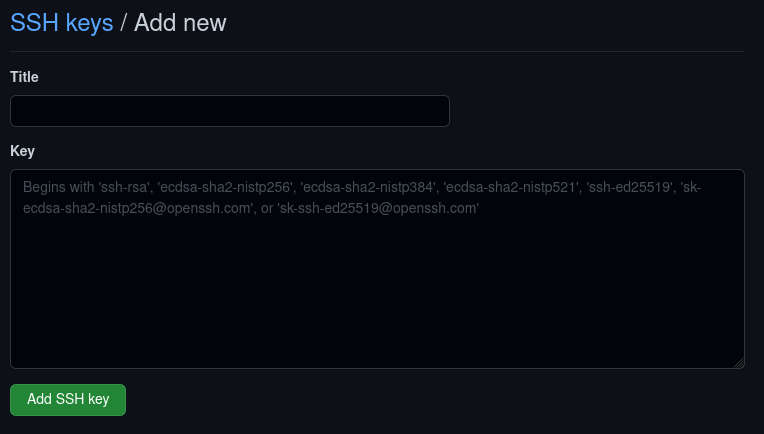
\includegraphics[width=0.75\textwidth]{./imgs/add_ssh.png}
\end{figure}

%%%%%%%%%%%%%%%%%%%%%%%%%%%%%%%%%%%%%%%%%%%%%%%%%%%%%%%%%%%%%%%%%%%%%%%%%%%%%%%%%%%%%%%%%%%%%%%%
\section{Cloning a Repository}

Today we will be practicing with the assignment that can be found at the following link: \\
\begin{lstlisting}
https://classroom.github.com/a/hdmi4qND
\end{lstlisting}
In clicking on this link a repository will be generated on your GitHub account according to a template. In order to modify this repository on our local machine we must first \textbf{clone} the repository. To do this, navigate to the newly generated repository and  (1)click on the code then (2) click on the clipboard to copy the SSH link.
\begin{figure}[H]
  \centering
  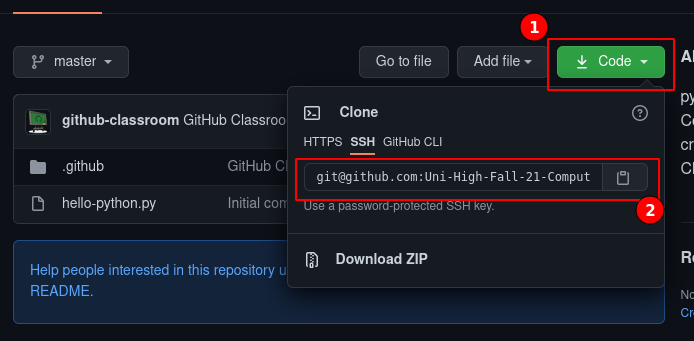
\includegraphics[width=0.75\textwidth]{./imgs/cloning.png}
\end{figure}
Then, using the terminal, navigate to the directory that you want to clone the repository to, and execute the following command being sure to replace it \lstinline|[url]| with the URL associated with your repo.

\begin{lstlisting}[language=bash]
$ cd <directory path>
$ git clone [url]
\end{lstlisting}

By default, this repository should have the following elements:
\begin{itemize}
  \item README.md \textrightarrow This ReadMe file is where you can store and display information associated with the repository which will be rendered on the associated repo's page.
  \item hello-python.py \textrightarrow This is the Python file that we will be modifying, adding, committing, and pushing.
\end{itemize}

%%%%%%%%%%%%%%%%%%%%%%%%%%%%%%%%%%%%%%%%%%%%%%%%%%%%%%%%%%%%%%%%%%%%%%%%%%%%%%%%%%%%%%%%%%%%%%%%
\section{Modifying the Files}

\subsection{README.md}

For the final portion of the lab you will be creating and them modifying the \lstinline|README.md| and \lstinline|hello-python.py| files. Follow these instructions with regard to the README.md file:
\begin{enumerate}
  \item Create and then open the README.md file in your text editor of choice and add a header and some information on the project. Refer to the markdown reference page for the syntax to achieve this.
  \item Add this file to the index via the following command:
\begin{lstlisting}[language=bash]
$ git add README.md
\end{lstlisting}
  \item Now that a snapshot of the updated file has been added to the index we now want to commit this change. In doing this we create a type of checkpoint that could be reverted to at a later date if need be:
\begin{lstlisting}[language=bash]
$ git commit -m "Updated README.md"
\end{lstlisting}
\item Now that this file has been committed locally we now want to push our changes to the remote version of our repo to (1) keep our latest changes backed up and (2) allow others to see the latest version:
\begin{lstlisting}[language=bash]
$ git push origin master
\end{lstlisting}
\end{enumerate}

Now that we have updated our README.md file you can visit the repo on GitHub and view the changes.

\subsection{hello-python.py}

Now we will apply a similar process to modify and update the hello-python file:
\begin{enumerate}
  \item Open the \lstinline|hello-python.py| file and modify it such that outputs \lstinline|Hello, World!| to the terminal. This can be tested via the following command on line 1 and should produce the output displayed on the second line:
\begin{lstlisting}[language=bash]
$ python hello-python.py
> Hello, World!
\end{lstlisting}
  \item Add this file to the index.
  \item Commit the file and enter an appropriate commit message.
  \item Push the file to the master branch.
  \item This repo is attached to an autograder on GitHub classroom. In order to determine if you have completed this stage of the assignment correctly visit the GitHub classroom website to view the autograder test cases.
\end{enumerate}

%%%%%%%%%%%%%%%%%%%%%%%%%%%%%%%%%%%%%%%%%%%%%%%%%%%%%%%%%%%%%%%%%%%%%%%%%%%%%%%%%%%%%%%%%%%%%%%%

\newpage
\section{Key Git Terms}

Commands:
\begin{enumerate}
  \item \textbf{git clone [url]:} Makes a local copy of a remote repository on your machine.
  \item \textbf{git add [options] [file]:} Adds a file or a series of files and their contents to the \textit{index}.
  \item \textbf{git reset [file]: } Unstages a file or, if no file is specified, all files from the index.
  \item \textbf{git status: } Shows you files that are tracked/untracked as well as those that are staged for commit.
  \item \textbf{git commit -m ``message'': } Makes a commit to the version history with an associated message that is included in quotes after the -m tag.
  \item \textbf{git pull: } Pulls changes from remote version history.
  \item \textbf{git push [remote] [branch]: } Pushes the local version of your git history to a specified remote/branch.
\end{enumerate}

Terms:
\begin{enumerate}
  \item \textbf{index: } A snapshot of the current files to be used in the next commit.
  \item \textbf{unstage/staged: } When files are added to the index we refer to them as being ``staged'' for the next commit. When they are removed we refer to this as unstaging.
  \item \textbf{tracked/untracked: } Files that are tracked are those that are being tracked for changes by git. Those files that are untracked are not currently apart of your version history and are not being tracked for changes.
\end{enumerate}


\section{Markdown Reference}

\begin{figure}[H]
  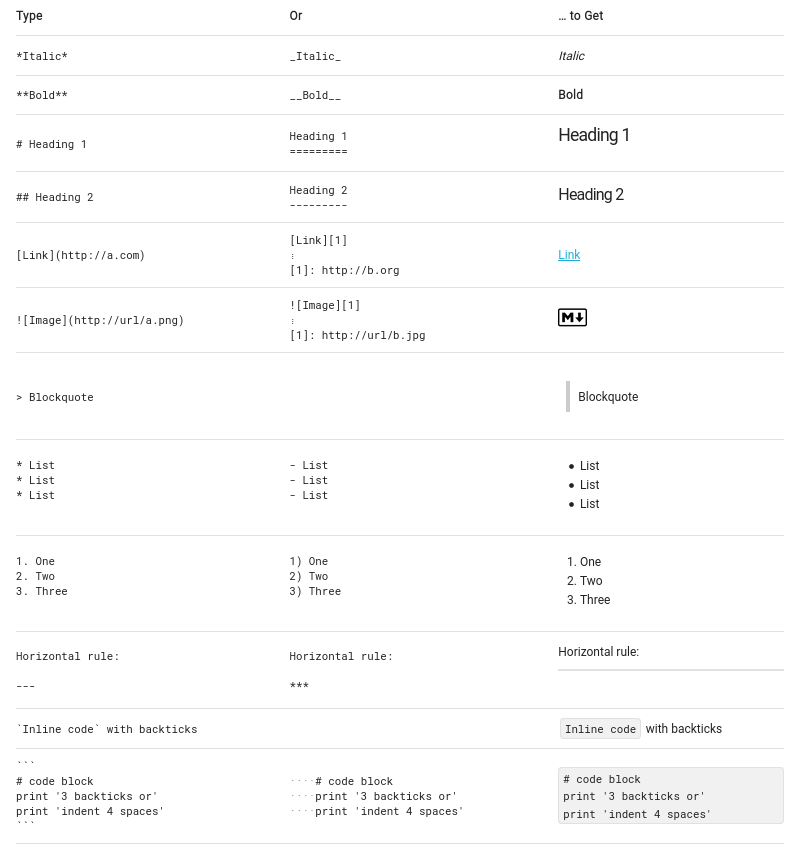
\includegraphics[width=\textwidth]{./imgs/markdown.png}
\end{figure}

Link to reference page: https://commonmark.org/help/















\end{document}
